\documentclass{standalone}
\usepackage{tikz}
\usepackage{ctex,siunitx}
\setCJKmainfont{Noto Serif CJK SC}
\usepackage{tkz-euclide}
\usepackage{amsmath}
\usetikzlibrary{patterns, calc,3d}
\usetikzlibrary {decorations.pathmorphing,decorations.pathreplacing,decorations.shapes}
\begin{document}
\small
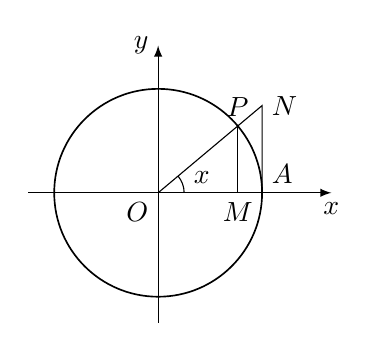
\begin{tikzpicture}[>=latex,scale=1.1]
  \draw[->](-1.5,0)--(2.0,0)node[below]{$x$};
  \draw[->](0,-1.5)--(0,1.7)node[left]{$y$};
  \node at (0,0)[below left]{$O$};
  \draw[semithick](0,0)circle(1.2);
  \draw(0,0)--(1.2,{1.2*tan(40)})node[right]{$N$}--(1.2,0)node[above right]{$A$};
  \draw(40:1.2)node[above]{$P$}--({1.2*cos(40)},0)node[below]{$M$};
  \draw(0.3,0)arc(0:40:0.3)node[at start,above right]{$x$};
\end{tikzpicture}
\end{document}